%%%%%%%%%%%%%%%%%% LEGENDRE EQUATION %%%%%%%%%%%%%%%%%%

\newcommand{\Legendre}[1]
{
	\onegraph{$x$}{$y(x)$}{ no marks, xmax = 1, xmin = -1}
	%
	{./doc/chapters/Boundary_Value_Problem/figures/Legendre.plt}{ }{1}{ #1 }
}

\newcommand{\LegendreError}[1]
{
	\onegraph{$x$}{$E(x)$}{ no marks, xmax = 1, xmin = -1}
	%
	{./doc/chapters/Boundary_Value_Problem/figures/Legendre_Error.plt}{ }{1}{ #1 }
}



%%%%%%%%%%%%%%%%%% LINEAR PLATE %%%%%%%%%%%%%%%%%%

\newcommand{\LinearPlate}[1]
{   
	\onecontour{ xlabel = $x$, ylabel = $y$, colormap/bluered}{21}
	%
	{./doc/chapters/Boundary_Value_Problem/figures/Linear_Plate_2D.dat}{}{ #1 }
}

\newcommand{\LinearPlateError}[1]
{   
	\onecontour{ xlabel = $x$, ylabel = $y$, colormap/bluered}{21}
	%
	{./doc/chapters/Boundary_Value_Problem/figures/Linear_Plate_2D_Error.dat}{}{ #1 }
}


%%%%%%%%%%%%%%%%%% NON LINEAR PLATE %%%%%%%%%%%%%%%%%%

\newcommand{\NonLinearPlate}[1]
{   
	\onecontour{ xlabel = $x$, ylabel = $y$, colormap/bluered}{11}
	%
	{./doc/chapters/Boundary_Value_Problem/figures/Non_Linear_Plate_2D.dat}{}{ #1 }
}

\newcommand{\NonLinearPlateStress}[1]
{   
	\onecontour{ xlabel = $x$, ylabel = $y$, colormap/bluered}{11}
	%
	{./doc/chapters/Boundary_Value_Problem/figures/Non_Linear_Plate_2D_Stress.dat}{}{ #1 }
}

%%%%%%%%%%%%%%%%%% DEVELOPER FIGURES %%%%%%%%%%%%%%%%


\newcommand{\BVPlinearity}
{
	\begin{figure}[htpb]
		\centering
		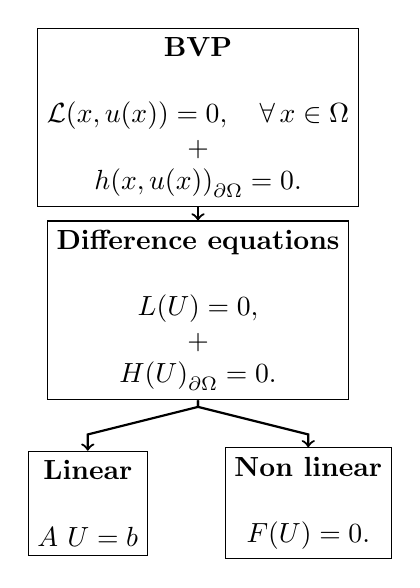
\begin{tikzpicture}[scale=0.7]   	
		
		\tikzstyle{every node}=[draw, align=center, rectangle ]
		
		\node(a) at (0,0) {\textbf{BVP} \\ \\
			$ \vect{\mathcal{L}}(\vect{x},\vect{u}(\vect{x}))= \vect{0}, \quad \forall \, \vect{x} \in \Omega $ \\ 
			+ \\ 
			$\eval{\vect{h}(\vect{x},\vect{u}(\vect{x}))}_{\partial \Omega} = 0.$};
		
		\node(b) at (0,-3.5) {\textbf{Difference equations} \\ \\
			$ L(U) = 0, $ \\ 
			+ \\ 
			$\eval{H(U)}_{\partial \Omega} = 0.$};
		
		\node(c) at (-2,-7) {\textbf{Linear} \\ \\
			$ A \ U =  \vect{b} $  };
		
		\node(d) at (2,-7) {\textbf{Non linear} \\ \\
			$ F(U) = 0.$};
		
		\draw [->, thick = 1 pt] (a) -- (b) ;
		\draw [->, thick = 1 pt] (b) -- (0,-5.25) -- (-2,-5.75) -- (c);
		\draw [->, thick = 1 pt] (b) -- (0,-5.25) --  (2,-5.75) -- (d);
		\end{tikzpicture}
		\caption{Linear and non linear boundary value problems.}
		\label{fig:BVPlinearity}
	\end{figure}
}